\documentclass{beamer}
\usetheme{Madrid}
\usepackage[utf8]{inputenc}

\usepackage{xcolor}
%Information to be included in the title page:
\title{Densities of $k$ Parent Aliquot Numbers}
\author{Gavin Guinn}
\institute{University of Calgary}
\date{June, 2020}
\usepackage{graphicx} %package to manage images

\makeatletter
\newcommand{\subalign}[1]{%
  \vcenter{%
    \Let@ \restore@math@cr \default@tag
    \baselineskip\fontdimen10 \scriptfont\tw@
    \advance\baselineskip\fontdimen12 \scriptfont\tw@
    \lineskip\thr@@\fontdimen8 \scriptfont\thr@@
    \lineskiplimit\lineskip
    \ialign{\hfil$\m@th\scriptstyle##$&$\m@th\scriptstyle{}##$\hfil\crcr
      #1\crcr   
    }%
  }%
}
\makeatother


\begin{document}



\newcommand\blfootnote[1]{%
  \begingroup
  \renewcommand\thefootnote{}\footnote{#1}%
  \addtocounter{footnote}{-1}%
  \endgroup
}

\frame{\titlepage}

\begin{frame}{Overview}
\tableofcontents
\end{frame}

\section{Aliquot Sequences}
\begin{frame}
\frametitle{Aliquot Sequences}

\begin{block}{Sum of Divisors}
For any natural number $n$ the sum of divisors of $n$ is defined
$\sigma(n) = \sum_{d|n} d$
\end{block}

And its close relative the sum of proper divisor function
\begin{block}{Sum of Proper Divisors}
$s(n) = \sigma(n) - n$
\end{block}
If $s(m) = n$ then $m$ is known as the parent of $n$ and $n$ is referred to as \textit{aliquot}. It is possible that $n$ could have multiple parents.  \linebreak \linebreak
A number not in the image of $s(\cdot)$ is known as \textit{non-aliquot} or more colourfully as an \textit{aliquot orphan}
\end{frame}

\begin{frame}
\frametitle{Aliquot Sequences, cont.}
An aliquot sequence is the iteration of $s(n)$
\begin{align*}
    s(10) &= 1 + 2 + 5\\  
    s(8) &= 1 + 2 + 4\\
    s(7) &= 1\\
    s(1) &= 0
\end{align*}

Above is an example of a sequence terminating after hitting a prime.\linebreak\linebreak
Sequences can also enter a cycle on a perfect number:
$$s(8128) \to s(8128) \to ...$$
Or enter a cycle of \textit{sociable numbers}: { \tiny \begin{align*} 
    &s(\mathbf{14316}) \to s(19116) \to s(31704) \to s(47616) \to s(83328) \to s(177792) \to s(295488) \to s(629072) \to s(589786) \to \\
    &s(294896) \to s(358336) \to s(418904) \to s(366556) \to s(274924) \to s(275444) \to s(243760) \to s(376736) \to s(381028) \to \\
    &s(285778) \to s(152990) \to s(122410) \to s(97946) \to s(48976) \to s(45946) \to s(22976) \to s(22744) \to s(19916) \to\\ 
    &s(17716) \to s(\mathbf{14316})
\end{align*}} 
\end{frame}


\begin{frame}{Aliquot Sequences, cont.}
It is an open question whether all aliquot sequences converge
\begin{block}{Catalan-Dickson Conjecture}
Every aliquot sequence ends in a prime, a perfect number, or a set of sociable numbers.
\end{block}
However many seem to diverge, such as the sequence starting with $s(276)$

\begin{block}{Guy-Selfridge Counter Conjecture}
    An infinite amount of aliquot sequences are unbounded 
\end{block}
\end{frame}
\begin{frame}{Aliquot Sequences, cont.}
     \begin{figure}[h]
     \centering
     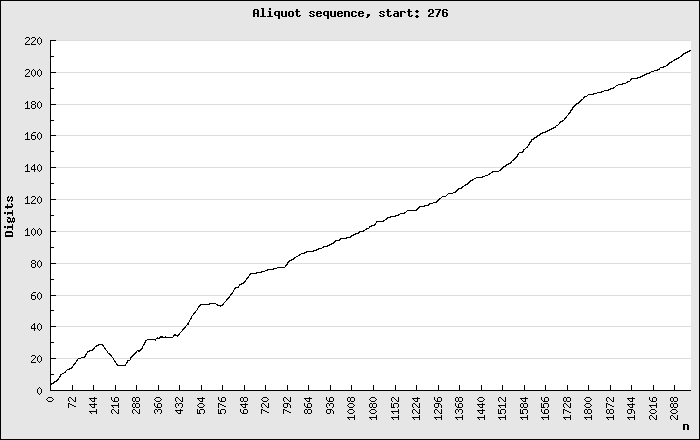
\includegraphics[width=.9\textwidth]{aliquot.png}
     \caption{Growth of the sequence starting with $s(276)$, from \textcolor{blue}{\cite{aliqSeq}}}
    \end{figure}
\end{frame}

\begin{frame}
\frametitle{Natural Density}
For some sequence $S$ of positive integers define a counting function $A(x) = |\{n \in S : 1 \leq n \leq x\}|$ 
\begin{block}{Natural Density of Sequence $S$}
$$d(S)=\lim_{x\to\infty} \frac{A(x)}{x}$$
\end{block}

The additive property of natural density will come in handy  
\begin{block}{Additive Property of Natural Density}
Let $S_1, S_2$ be disjoint sequences with natural density, then: $$d(S_1 \cup S_2) = d(S_1) + d(S_2)$$
\end{block}
\end{frame}


\begin{frame}{Motivation from Dr.Guy}

\small{Think of a number!! Say 36\%, which is nice and divisible. It appears that about 36\% of the even numbers are "orphans". \linebreak

Divide by 1. For about 36\% of the (even) values of n there is just one positive integer m such that s(m) = n. These values of n have just one "parent". \linebreak

Divide by 2.  About 18\% of the even values of n have exactly two parents. \linebreak

Divide by 3. About 6\% of the even values of n have three parents. \linebreak

Divide by 4. About 1 1/2 \% of the even values of n have just 4 parents.  \linebreak

This suggests that 1/(p! e) of the even numbers have p parents.\linebreak

Experiments suggests that these values are a bit large for small values of p and a bit small for larger values of p. Can anything be proved?\\}
\end{frame}

\begin{frame}
\frametitle{Density of Aliquot Orphans}

Let $\Delta_k$ be the natural density of $k$ parent aliquot numbers.\linebreak \linebreak
Dr. Guy's observations suggest the densities of aliquot orphans are a specific instance of the more general $\Delta_k$ \linebreak\linebreak
These slides first present the heuristic model for the density of aliquot orphans proposed by Pollack and Pomerance \textcolor{blue}{\cite{pollPom}} then continues to present my work in generalizing that model
\begin{block}{Density of Non-Aliquot Numbers (3.4)}
$$\Delta = \lim_{y \to \infty}\frac{1}{\log y} \sum_{\substack{a\leq y \\ 2 | a}} \frac{1}{a}\text{e}^{-a/s(a)}$$
\end{block}

\end{frame}






% \section{Density of Aliquot Orphans}
% \begin{frame}
% \frametitle{Aliquot Orphans}
% Pollack and Pomerance \textcolor{blue}{\cite{pollPom}} propose a probabilistic model for the density of non-aliquot numbers
% \begin{block}{Density of Non-Aliquot Numbers (3.4)}
% $$\Delta = \lim_{y \to \infty}\frac{1}{\log y} \sum_{\substack{a\leq y \\ 2 | a}} \frac{1}{a}\text{e}^{-a/s(a)}$$
% \end{block}
% To understand this it is instructive to look at an intermediate expression for $\Delta$
% \end{frame}


\begin{frame}
\frametitle{Density of Aliquot Orphans, cont.}
To understand this model it is instructive to look at an intermediate expression for $\Delta$
\begin{block}{Density of Non-Aliquot Numbers (3.1)}
$$\Delta = \lim_{y \to \infty} \frac{\phi(A_y)}{A_y} \sum_{\substack{a\leq y \\ 2 | a}} \frac{1}{a} e^{-a/s(a)}$$
\end{block}
\begin{itemize}
    \item $\phi(x)$ is Euler's totient function 
    \item $s(x)$ is the sum-of-proper-divisors function
    \item $A_y = \text{ lcm}[1, 2, ..., y]$
\end{itemize}
\end{frame}




\begin{frame}
\frametitle{Density of Aliquot Orphans, cont.}
From here I will be presenting my understanding of how the authors constructed an expression for $\Delta$ (3.1).\linebreak
\linebreak
To find the density of non-aliquot numbers the authors construct a series of disjoint subsets, let:
$$A_y = \text{ lcm}[1, 2, ..., y]$$
Then for a positive integer $a | A_y$, let:
$$T_a = \{n : \text{gcd}(n, A_y) = a\}$$
We also bound the set: $$T_a(x) = T_a \cap [1,x]$$
\end{frame}

\begin{frame}{Density of Aliquot Orphans, cont.}
A useful property of how these sets $T_a$ are constructed is that the parity of $a$ determines the parity of everything in the set; its worth quickly proving this for later use.\linebreak\linebreak
    \textbf{Claim:} If $a$ is even then $n$ must also be even.\\
   \textbf{Proof:} Assume $a$ is even, then: 
    $$\text{gcd}(n, A_y) = a = 2b$$
    So  $2b|n$ which proves the claim.\\
   
    
\end{frame}



\begin{frame}{Aliquot Orphans, cont}

    \textbf{Claim:} If $a$ is odd then $n$ is also odd\\
    \textbf{Proof:} Assume $a$ is odd, also noting that for $y \geq 2$ that $2|A_y$, so we have: 
    \begin{align*}
        \text{gcd}(n, A_y) &= a\\
        \text{gcd}(n, 2c) &= 2b+1
    \end{align*}

    For contradiction assume that $n$ is even, then:
     $$\text{gcd}(2d, 2c) = 2b+1$$
    But $\text{gcd}(kr, km) = k\cdot \text{gcd}(r, m)$  which gives: \textcolor{blue}{\cite{gcd}}
    $$2 \cdot \text{gcd}(d, c) = 2b+1$$
    This contradiction implies that $n$ must be odd, establishing the claim
   
\end{frame} 



\begin{frame}
\frametitle{Aliquot Orphans, cont.}
   We have a series of disjoint subsets $T_a$, next we determine what proportion of each set are orphans. We need to setup some assumptions to use statistical tools to handle this problem:
\begin{itemize}
    \item Assume that $s(\cdot)$ maps $T_a$ to $T_a$ for each $a | A_y$ (Asymptotically true if $n > e^{e^y}$ and $y \to \infty$)
    \item Assume that for $n \in T_a $ that we have $\sigma(n)/n \approx \sigma(a)/a $ (Asymptotically true up to sets of vanishing density as $y \to \infty$)
    \item Assume that $s(\cdot)$ is a random map
\end{itemize}
\end{frame}

\begin{frame}
\frametitle{Aliquot Orphans, cont.}
The classic "balls and bins"  statistics problem \textcolor{blue}{\cite{ballsBins}} comes in handy here.  Say that we have $n$ bins and decide to toss $m$ balls independently and randomly into those bins. 
\begin{block}{Probability of a Empty Bin}
{\large$$ \mathbb{P}[\text{bin } i \text{ empty}] = (1- \frac{1}{n})^m$$}
\end{block}

\begin{block}{Number of a Empty Bins}
{\large$$ \# [\text{empty bins}] = n(1- \frac{1}{n})^m$$}
\end{block}
\end{frame}

\begin{frame}
\frametitle{Aliquot Orphans, cont.}
Using that model to estimate the proportion of non-aliquot numbers in a specific set $T_a$, naturally: $$\text{\# bins} = |T_a(x)|$$
Next we need an analog for the number of balls, a set $B$ such that $m \in B$ if and only if $s(m) \in T_a(x)$  \linebreak \linebreak
Previously we assumed that $s(\cdot)$ maps $T_a$ back into $T_a$ so we know that $B \subset T_a$
\end{frame}

\begin{frame}
\frametitle{Aliquot Orphans, cont.}
Its worth noting that $\frac{a}{s(a)}$ provides a measure of how much smaller or larger $a$ is compared to $s(a)$. By assumption every element in $T_a$ also shares this same approximate ratio as: $$\frac{a}{s(a)} = \frac{1}{(\sigma(a)/a)-1}$$
We can use this fact to find the range of values of that will map into $T_a(x)$ by: $$x \left(\frac{a}{s(a)}\right) = \frac{x}{(\sigma(a)/a)-1}$$


For instance let $a = 2$ and $x=100$ then: $$100\left( \frac{2}{s(2)}\right) = 200$$

So in this case $s(m)$ will map into $T_2(100)$ if and only if $m \in T_2(200)$

%We can utilize the fact that all elements in $T_a$ have around the same abundance or deficiency to find a bound relative to $x$ 
%Since every element in $T_a$ shares similar abundance or deficiency we can observe that the largest element that will map into $T_a(x)$ will come from  
\end{frame}

% \begin{frame}
% \frametitle{Aliquot Orphans, cont.}
% We know $X \subset T_a$ so next it would be nice to find a value $y$ such that $T_a(y) = B $ \linebreak 


% Previously we assumed $\forall n \in T_a$ that: $$\frac{\sigma(a)}{a} \approx \frac{\sigma(n)}{n}$$
% So $\frac{\sigma(a)}{a}$ is a approximate measure of \textit{abundance} or \textit{deficiency} for every element in $T_a$ 
% \end{frame}




% \begin{frame}
% \frametitle{Aliquot Orphans, cont.}
% Assume that $a$ is even. If $s(m) \in T_a(x)$ then by assumption we have that $m \in T_a$. Since for all $n \in T_a $ we have $$\frac{\sigma(a)}{a} \approx \frac{\sigma(n)}{n}$$ It would instructive to have a measure of abundance or of deficiency for everything in $T_a$ so we could have a bound for the range of values that $s$ will map into $T_a(x)$.  One way to do this would be: $$x \left(\frac{a}{s(a)}\right) = \frac{x}{(\sigma(a)/a)-1}$$ For instance let $a = 2$ and $x=100$ then: $$100\left( \frac{2}{s(2)}\right) = 200$$
% Since everything in the set $T_2$ is deficient by a factor of about $2$ the maximum value such that $s(m) \in T_a(100)$ must be $m \leq 200$
% \end{frame}

\begin{frame}
\frametitle{Aliquot Orphans, cont.}
So we have a number of 'bins': $$n = |T_a(x)|$$ 
And the number of 'balls': $$m = |T_a\left(\frac{x\cdot a}{s(a)} \right)|$$ 
Plugging those values in: $$\left(1-\frac{1}{n}\right)^m = \left(1-\frac{1}{|T_a(x)|}\right)^{|T_a(x\cdot a/s(a))|} $$
Which is the probability of any specific element in $T_a(x)$ being non-aliquot
\end{frame}

\begin{frame}
\frametitle{Aliquot Orphans, cont.}

The authors observe that: \blfootnote{Where $f(x) \sim g(x) \iff \lim_{x \to \infty} f(x)/g(x) = 1$}$$|T_a(x)|  \sim  \frac{\phi(A_y) \cdot x}{ A_y \cdot a}$$ So we can substitute in: 
$$ \left(1-\frac{1}{|T_a(x)|}\right)^{|T_a(x\cdot a/s(a))|} = \left(1-\frac{1}{\left(\frac{\phi(A_y) \cdot x}{ A_y \cdot a}\right)}\right)^{(\phi(A_y) \cdot x)/( A_y \cdot s(a))}$$
\end{frame}

\begin{frame}{Asymp. Equiv.}
The authors observe that:
    $$|T_a(x)|  \sim  \frac{\phi(A_y) \cdot x}{ A_y \cdot a}$$
    Breaking this into terms we can make some observations about why this relation holds:
    $$\phi(A_y) = |\{n \in \mathbb{Z} \text{ } | \text{ gcd}(A_y,n) = 1 \text{ and } 1 \leq n \leq A_y \}|$$
    Euler's totient function counts the amount of numbers co-prime to its input up-to that input
    $$ \frac{\phi(A_y)}{ A_y }$$
    This is the ratio of numbers that are co-prime with $A_y$ upto $A_y$
\end{frame}

\begin{frame}{Asymp. Equiv.}
The core of the argument comes from the fact that: $$\text{gcd}(n, A_y) = 1 \implies \text{gcd}(an, A_y) = a  $$
\textbf{Proof:}\linebreak  
Assume that $\text{gcd}(n, A_y) = 1$, remember $a|A_y$ \begin{align*}
    \text{gcd}(an, A_y) &=  \text{gcd}(an, am) & \text{[$m>0$ and $m|A_y$]}\\
    &= a \cdot  \text{gcd}(n, m) & \text{[gcd$(ax,ay)$ = $a \cdot \text{gcd}(x,y)$]}
\end{align*}

So to get the result all we need to show is $\text{gcd}(n, m) = 1$ we can use another gcd property to establish this: $$\text{gcd}(x, yz) = 1 \iff \text{gcd}(x, y) = 1 \text{ and } \text{gcd}(x, z) = 1$$
    
\end{frame}

\begin{frame}{Asymp. Equiv.}
Plugging values into the bi-conditional:
$$\text{gcd}(n, A_y) = \text{gcd}(n, am) = 1 \iff \text{gcd}(n, a) = 1 \text{ and } \text{gcd}(n, m) = 1$$

By assumption we know $\text{gcd}(n, am) = 1$ it follows that: $$\text{gcd}(n, a) = 1 \text{ and } \text{gcd}(n, m) = 1$$ 

So $a \cdot  \text{gcd}(n, m) = a$ which is sufficient to establish the implication:
$$\text{gcd}(n, A_y) = 1 \implies \text{gcd}(an, A_y) = a$$
\end{frame}

\begin{frame}{Asymp Equiv}
    While we have that: $$\text{gcd}(n, A_y) = 1 \implies \text{gcd}(an, A_y) = a$$
    It is not true that: $$ \text{gcd}(an, A_y) = a  \implies \text{gcd}(n, A_y) = 1$$
    As a consequence of this we know that every $n$ such that $n \leq A_y$ and $gcd(n, A_y) = 1$ must correspond to a member of the set $T_a(A_y \cdot a)$. \linebreak \linebreak  However there exists elements in $T_a$ that do not correspond to the totatives of $A_y$. The table on the next slide outlines some examples of this case in \textcolor{blue}{blue}.
\end{frame}

\begin{frame}{Asymp. Equiv.}
\begin{center}
\begin{table}[]
    \centering
    \begin{tabular}{| c | c | l || c | c | l|}
\hline
 $n$ & $T_3$ & Type & $n$ & $T_3$ & Type \\
 \hline
1                       & 3                     & $3 \cdot 1$           & 31                      & 93                      & $3 \cdot 31$\\
\textcolor{blue}{NA}    & \textcolor{blue}{9}   & $3 \cdot 3^1$         & \textcolor{blue}{NA}    & \textcolor{blue}{99}    & $3 \cdot (3 \cdot 11)$\\
7                       & 21                    & $3 \cdot 7$           & 37                      & 111                     & $3 \cdot 37$\\
\textcolor{blue}{NA}    & \textcolor{blue}{27}  & $3 \cdot 3^2$         & \textcolor{blue}{NA}    & \textcolor{blue}{117}   & $3 \cdot (3 \cdot 13)$\\
11                      & 33                    & $3 \cdot 11$          & 41                      & 123                     & $3 \cdot 41$\\
13                      & 39                    & $3 \cdot 13$          & 43                      & 129                     & $3 \cdot 43$\\
17                      & 51                    & $3 \cdot 17$          & 47                      & 141                     & $3 \cdot 47$\\
19                      & 57                    & $3 \cdot 19$          & 49                      & 147                     & $3 \cdot 49$\\
\textcolor{blue}{NA}    & \textcolor{blue}{63}  & $3 \cdot (3 \cdot 7)$ & \textcolor{blue}{NA}    & \textcolor{blue}{153}   & $3 \cdot (3 \cdot 17)$\\
23                      & 69                    & $3 \cdot 23$          & 53                      & 159                     & $3 \cdot 53$\\
\textcolor{blue}{NA}    & \textcolor{blue}{81}  & $3 \cdot 3^3$          & \textcolor{blue}{NA}    & \textcolor{blue}{171}   & $3 \cdot (3 \cdot 19)$\\
29                      & 87                    & $3 \cdot 31$          & 59                      & 177                     & $3 \cdot 59$\\


\hline
\end{tabular}
\end{table}

\end{center}
\begin{itemize}
    \item $A_y = \text{lcm}(1,2,3,4,5) = 60$ 
    \item $n \text{ s.t. gcd}(n, A_y) = 1$ 
    \item $T_3 = \{n \text{ }| \text{ }\text{gcd}(n, A_y) = 3\}$
\end{itemize}
    

\end{frame}

\begin{frame}{Asymp. Equiv.}
    So where does this leave us in proving:
    $$|T_a(x)|  \sim  \frac{\phi(A_y) \cdot x}{ A_y \cdot a}$$
    I am not precisely sure, we are to show that:
    $$\lim_{x \to \infty} \frac{|T_a(x)|}{\left(\frac{\phi(A_y) \cdot x}{ A_y \cdot a}\right)} =1$$
    And we know that: $$\frac{\phi(A_y) \cdot A_y \cdot a}{ A_y \cdot a} \neq |T_a(A_y \cdot a)|$$
    As: $$\frac{\phi(60) \cdot 180}{ 60 \cdot 3} = 16 \neq  24 = |T_3(180)|$$
\end{frame}

\begin{frame}{Asymp. Equiv.}
    My next step when I continue looking into this will be to prove:$$\text{gcd}(x, A_y) = a $$
     \begin{center}
        \underline{if and only if}
    \end{center}
    $$x = an \text{ and } \text{gcd}(a, n ) = 1$$
    \begin{center}
        \underline{or}
    \end{center}
    $$x = a^i, \text{ } i \geq 1$$
    \begin{center}
        \underline{or}
    \end{center}
    $$x = a^2n$$
    
    Where $n \perp A_y$ and $n \leq A_y$ \linebreak \linebreak
    I know this statement is flawed as it doesn't account for $x > A_y \cdot a$, I will fix that later. The idea is to separate into classes.
\end{frame}

\begin{frame}{Rabbit}
     \begin{figure}[h]
     \centering
     \includegraphics[width=.8\textwidth]{rabbit.jpg}
    \caption{Bounty Reward Rabbit}       
    \end{figure}
\end{frame}


\begin{frame}{Asymp. Equiv.}
So next we would like to find what proportion of numbers $n$ such that:$$\text{gcd}(an, A_y) = a$$ 
Well on top of the ratio we will have: $$\phi(A_y)$$
As this number counts how many solutions we have to $\text{gcd}(an, A_y) = a$. Then what goes in the denominator? We are looking for the ratio of $\#an$ that satisfies the equation over all possible values of $\#an$. Since earlier we defined $n \leq A_y$ so naturally $an \leq aA_y$ we can use $aA_y$ as the denominator of the ratio. 
  
\end{frame}

\begin{frame}{Asymp. Equiv.}
So we have: $$\frac{\phi(A_y)}{aA_y}$$ as the proption of solutions
\end{frame}

\begin{frame}
\frametitle{Aliquot Orphans, cont.}
We are looking for information about the asymptotic behaviour of this probability:
\begin{align*}
    &\lim_{x \to \infty}\left(1-\frac{1}{\left(\frac{\phi(A_y) \cdot x}{ A_y \cdot a}\right)}\right)^{(\phi(A_y) \cdot x)/( A_y \cdot s(a))}\\
    &= e^{-a/s(a)}
\end{align*}
Which is the probability of any element in $T_a$ being non-aliquot
\blfootnote{Note: $\lim_{x \to \infty} (1- \frac{1}{x})^x = e$}
\end{frame}


\begin{frame}
\frametitle{Aliquot Orphans, cont.}
Working heuristically, since:  $$|T_a(x)|  \sim  \frac{\phi(A_y) \cdot x}{ A_y \cdot a}$$ So we treat $\phi(A_y)/ (a \cdot A_y) $ as the probability that any number is in $T_a$ (see \textcolor{blue}{\cite{density}} for a similar treatment)\linebreak
%that for any value of $x$ the proportion of integers in $T_a$ must be $\frac{\phi(A_y)}{ A_y \cdot a}$\\

So the probability that some number is both in $T_a$ and non-aliquot:
$$\frac{\phi(A_y)}{ A_y \cdot a} \cdot  e^{-a/s(a)}$$
\end{frame}

\begin{frame}
\frametitle{Image of $s(\cdot)$}
Let $p$ and $q$ be distinct primes. By the fundamental theorem of arithmetic the only divisors of $p \cdot q$ are in $\{1\text{, } p\text{, } q \text{, } pq\}$, so $s(pq) = 1 + p + q$.
\begin{block}{Goldbach Conjecture (Strong Variant)}
Every even number greater than 8 can be expressed as the sum of 2 distinct primes 
\end{block}
Assuming the stronger Goldbach Conjecture $\forall m \geq 4$ there exists unique primes $p$ and $q$ such that $2m = p + q$. $$s(pq) = 1 + p + q = 2m +1 $$
So every odd number greater than 8 is in the image of $s(\cdot)$,  \textbf{almost all odd numbers cannot be aliquot orphans}
\end{frame}

\begin{frame}\frametitle{Aliquot Orphans, cont.}
Since each set $T_a$ is disjoint we can apply the additive property of natural density to find the density of non-aliquot numbers over the positive integers: 
\begin{align*}
     \Delta &= \lim_{y \to \infty}  \sum_{\subalign{a&|A_y\\2&|a}} \frac{\phi(A_y)}{a \cdot A_y} \cdot e^{-a/s(a)}\\ \\
     &= \lim_{y \to \infty} \frac{\phi(A_y)}{A_y} \sum_{\subalign{a&|A_y \\ 2 &| a}} \frac{1}{a} e^{-a/s(a)}
\end{align*}
We restrict $a$ to even values as its parity determines the parity of everything in $T_a$ and we know that the density of odd aliquot orphans quickly vanishes
 
\end{frame}

\section{Densities $k$ Parent Aliquot Numbers }
\begin{frame}{$k$ Parent Aliquot Numbers }
So how do we extend this reasoning to count aliquot numbers with $k$ parents?
    \begin{block}{Probability of a Bin Containing $k$ Balls}
        $$\mathbb{P}[k \text{ balls in bin}] = {m \choose k } \frac{1}{n^k} (1- \frac{1}{n})^{m-k}$$
        \begin{itemize}
            \item $k$ is the number of balls in a bin
            \item $n$ is the number of bins
            \item $m$ is the number of balls
        \end{itemize}

    \end{block}

\end{frame}

\begin{frame}{$k$ Parent Aliquot Numbers}
Using the same values of: \begin{align*}
    &n = \frac{\phi(A_y) \cdot x}{ A_y \cdot a} & &m = \frac{\phi(A_y) \cdot x}{A_y \cdot s(a)}
\end{align*}
Plugging those in we get:  $$\mathbb{P}[k \text{ parents}] =  \lim_{x \to \infty}{\frac{\phi(A_y) \cdot x}{A_y \cdot s(a)} \choose k } \frac{1}{\left(\frac{\phi(A_y) \cdot x}{ A_y \cdot a}\right)^k} \left(1- \frac{1}{\left(\frac{\phi(A_y) \cdot x}{ A_y \cdot a}\right)}\right)^{\frac{\phi(A_y) \cdot x}{A_y \cdot s(a)  } -k}$$

Which is the probability of a specific number in $T_a$ having $k$ parents
\end{frame}

% \begin{frame}{$k$ Parent Aliquot Numbers}
% I have evaluated this expression for a couple of values of $k$
% \begin{align*}
%     \mathbb{P}[0 \text{ parents}] &=  e^{-a/s(a)}\\\\
%   \mathbb{P}[1 \text{ parents}] &=  \frac{a}{s(a)} e^{-a/s(a)}\\\\
%     \mathbb{P}[2 \text{ parents}] &=    \frac{a^2}{2s(a)^{2}} e^{-a/s(a)}\\\\
%     \mathbb{P}[3 \text{ parents}] &=  \frac{a^3}{6s(a)^{3}} e^{-a/s(a)}
% \end{align*}
% \end{frame}

\begin{frame}{$k$ Parent Aliquot Numbers}
This probability cleans up quite nicely (proof excluded for brevity)
\begin{block}{Probability of an $n \in T_a$ having $k$ parents}
    $$\mathbb{P}[k \text{ parents}] = \frac{a^{k}}{k! \cdot s(a)^k} \cdot \text{e}^{-a/s(a)}$$
\end{block}

\begin{block}{Density of $k$ Parent Aliquot Numbers}
    $$\Delta_k = \lim_{y \to \infty} \frac{\phi(A_y)}{A_y} \sum_{a|A_{y}} \frac{a^{k-1}}{k! \cdot s(a)^k} \cdot \text{e}^{-a/s(a)}$$
 Note that this expression is not restricted to even values of $a$
\end{block}
\end{frame}

\begin{frame}{$k$ Parent Aliquot Numbers}
   The authors continue to establish an easier to compute expression for $\Delta$: \begin{align*}
       \Delta &= \lim_{y \to \infty} \frac{\phi(A_y)}{A_y} \sum_{\substack{a | A_y \\ 2 | a}} \frac{1}{a} e^{-a/s(a)} &(\text{3.1})\\ \\
       &= \lim_{y \to \infty} \frac{1}{\log y} \sum_{\substack{a\leq y \\ 2 | a}} \frac{1}{a} e^{-a/s(a)}&(\text{3.4})\\
   \end{align*} 
    Continuing the trend of unjustified claims this suggests:
    \begin{block}{Density of numbers with $k$ parents }
    
    $$\Delta_k = \lim_{y \to \infty} \frac{1}{\log y}\sum_{a \leq y} \frac{a^{k-1}}{k! \cdot s(a)^k} \cdot \text{e}^{-a/s(a)}$$
    \end{block}
\end{frame}

\begin{frame}{Tentative Numerical results}
\begin{center}
\begin{table}[]
    \centering
    \begin{tabular}{| c | c | c | c | c |}
\hline
 $y$ & $\Delta_0$ & $\Delta_1$ & $\Delta_2$ & $\Delta_3$ \\ 
 \hline
 \hline
 50000 & 0.163674852 & 0.211872977 & 0.150917967 & 0.091332510\\  
 100000 & 0.164576576 & 0.212205479 & 0.150682529 & 0.091010417\\
 150000 & 0.165055668 & 0.212382167 & 0.150556904 & 0.090837746\\
 200000 & 0.165376121 & 0.212500620 & 0.150473266 & 0.090722516 \\
250000 & 0.165614500 & 0.212588736 & 0.150411231 & 0.090637101\\
300000 & 0.165803078 & 0.212658477 & 0.150362014 & 0.090569168\\
\hline
\end{tabular}
    \caption{Approximate values of $\Delta_k$}
    \label{tab:my_label}
\end{table}

\end{center}
\end{frame}

\begin{frame}{Motivation from Dr.Guy}

\small{Think of a number!! Say 36\%, which is nice and divisible. It appears that about 36\% of the even numbers are "orphans". \linebreak

Divide by 1. For about 36\% of the (even) values of n there is just one positive integer m such that s(m) = n. These values of n have just one "parent". \linebreak

Divide by 2.  About 18\% of the even values of n have exactly two parents. \linebreak

Divide by 3. About 6\% of the even values of n have three parents. \linebreak

Divide by 4. About 1 1/2 \% of the even values of n have just 4 parents.  \linebreak

This suggests that 1/(p! e) of the even numbers have p parents.\linebreak

Experiments suggests that these values are a bit large for small values of p and a bit small for larger values of p. Can anything be proved?\\}
\end{frame}

\begin{frame}{Tentative Numerical results}
\begin{center}
{ \small
\begin{table}[]
    \centering
    \begin{tabular}{| c | c | c | c | c | c |}
\hline
 $y$ & $\Delta_0$ & $\Delta_1$ & $\Delta_2$ & $\Delta_3$ & $\Delta_4$ \\ 
 \hline

 50000 & 0.16367 & 0.16577 & 0.09741 & 0.04376 & 0.01651\\
100000 & 0.16458 & 0.16592 & 0.09714 & 0.04351 & 0.01637\\
150000 & 0.16506 & 0.16601 & 0.09699 & 0.04337 & 0.01630\\
200000 & 0.16538 & 0.16606 & 0.09689 & 0.04328 & 0.01625\\
250000 & 0.16561 & 0.16611 & 0.09682 & 0.04321 & 0.01622\\
300000 & 0.16580 & 0.16614 & 0.09676 & 0.04316 & 0.01619\\
\hline
\hline
\hline
 $1/(p! \cdot \text{e})$ & $1/(0! \cdot \text{e})$ & $1/(1! \cdot \text{e})$ & $1/(2! \cdot \text{e})$ & $1/(3! \cdot \text{e})$ & $1/(4! \cdot \text{e})$\\
 \hline
  - & 0.36787 & 0.36787 & 0.18393 & 0.06131 & 0.01532\\
 \hline
 \hline
  $1/2(p! \cdot \text{e})$ & $1/2(0! \cdot \text{e})$ & $1/2(1! \cdot \text{e})$ & $1/2(2! \cdot \text{e})$ & $1/2(3! \cdot \text{e})$ & $1/2(4! \cdot \text{e})$\\
 \hline
  - & 0.18393 & 0.18393 & 0.09196 & 0.03065 & 0.00766\\
  \hline

\end{tabular}
    \caption{Approximation of $\Delta_k$ (restricted to even $a$) compared to Dr. Guy's estimates}
    \label{tab:my_label}
\end{table}

}
\end{center}
{ \small
Where $\frac{1}{p! \cdot e}$ is the estimated density of $k$ parents aliquot numbers over the evens.\\ 
Where $\frac{1}{2(p! \cdot e)}$ is the estimated density of \textbf{even} $k$ parent aliquot numbers over all integers.}
\end{frame}



\section{Further Work}
\begin{frame}{Further work}
1) Compare estimates for $\Delta_k$ against numerical data on aliquot parents  \linebreak
2) Improve the computational accuracy of my estimates for $\Delta_k$  \linebreak
3) Prove: \begin{align*}
       \Delta_k &= \lim_{y \to \infty} \frac{\phi(A_y)}{A_y} \sum_{a|A_{y}} \frac{a^{k-1}}{k! \cdot s(a)^k} \cdot \text{e}^{-a/s(a)}\\
       &= \lim_{y \to \infty} \frac{1}{\log y}\sum_{a \leq y} \frac{a^{k-1}}{k! \cdot s(a)^k} \cdot \text{e}^{-a/s(a)}
   \end{align*}

\end{frame}

\section{References}
\begin{frame}{References}
    \begin{thebibliography}{9}
\setbeamertemplate{bibliography item}[text]

\bibitem{pollPom}
Paul Pollack, Carl Pomerance.
\textit{Some Problems of Erdős on the Sum-of-Divisors Function}. 
\texttt{https://math.dartmouth.edu/$\sim$carlp/btran10.pdf}

\bibitem{ballsBins} 
Hemanta Maji. 
\textit{Lecture 03: Balls \& Bins}.
\texttt{https://www.cs.purdue.edu/homes/hmaji/teaching/\\Spring\%202017/lectures/03.pdf}

\bibitem{aliqSeq} 
Paul Zimmermann.
\textit{Aliquot Sequences}.
\\\texttt{https://members.loria.fr/PZimmermann/records/aliquot.html}

\bibitem{gcd}
Franz Lemmermeyer.
\textit{Elementary Number Theory: Homework 2}.
\\\texttt{http://www.fen.bilkent.edu.tr/$\sim$franz/nth06/hwnt02a.pdf}

\bibitem{density}
Matthew Conroy.
\textit{Examples of integer sequence density calculations}.
\\\texttt{https://sites.math.washington.edu/$sim$conroy/WXML\\/integerSequenceNoise/density/densityExamples.pdf}


\end{thebibliography}
\end{frame}



\end{document}

\begin{frame}
\frametitle{Image of $s(\cdot)$}
Let $p$ and $q$ be distinct primes. By the fundamental theorem of arithmetic the only divisors of $p \cdot q$ are in $\{1\text{, } p\text{, } q \text{, } pq\}$, so $s(pq) = 1 + p + q$.
\begin{block}{Goldbach Conjecture (Strong Variant)}
Every even number greater than 8 can be expressed as the sum of 2 distinct primes 
\end{block}
Assuming the stronger Goldbach Conjecture $\forall m \geq 4$ there exists unique primes $p$ and $q$ such that $2m = p + q$. $$s(pq) = 1 + p + q = 2m +1 $$
So every odd number greater than 8 is in the image of $s(\cdot)$.
\end{frame}


\begin{frame}
\frametitle{Natural Density}
For some sequence $S$ of positive integers define a counting function $A(x) = |\{n \in S : 1 \leq n \leq x\}|$ 
\begin{block}{Natural Density of Sequence $S$}
$$d(S)=\lim_{x\to\infty} \frac{A(x)}{x}$$
\end{block}

The additive property of natural density will come in handy  
\begin{block}{Additive Property of Natural Density}
Let $S_1, S_2$ be disjoint sequences with natural density, then: $$d(S_1 \cup S_2) = d(S_1) + d(S_2)$$
\end{block}
\end{frame}


\section{Density of Aliquot Orphans}
\begin{frame}
\frametitle{Aliquot Orphans}
Pollack and Pomerance \textcolor{blue}{\cite{pollPom}} propose a probabilistic model for the density of non-aliquot numbers
\begin{block}{Density of Non-Aliquot Numbers (3.4)}
$$\Delta = \lim_{y \to \infty}\frac{1}{\log y} \sum_{\substack{a\leq y \\ 2 | a}} \frac{1}{a}\text{e}^{-a/s(a)}$$
\end{block}
To understand this it is instructive to look at an intermediate expression for $\Delta$
\end{frame}

\begin{frame}
\frametitle{Aliquot Orphans, cont.}
\begin{block}{Density of Non-Aliquot Numbers (3.1)}
$$\Delta = \lim_{y \to \infty} \frac{\phi(A_y)}{A_y} \sum_{\substack{a\leq y \\ 2 | a}} \frac{1}{a} e^{-a/s(a)}$$
\end{block}
\begin{itemize}
    \item $\phi(x)$ is Euler's totient function 
    \item $s(x)$ is the sum-of-proper-divisors function
    \item $A_y = \text{ lcm}[1, 2, ..., y]$
\end{itemize}


\end{frame}




\begin{frame}
\frametitle{Aliquot Orphans, cont.}
From here I will be presenting my understanding of how the authors constructed an expression for $\Delta$ (3.1).\linebreak
\linebreak
To find the density of non-aliquot numbers the authors construct a series of disjoint subsets, let:
$$A_y = \text{ lcm}[1, 2, ..., y]$$
Then for a positive integer $a | A_y$, let:
$$T_a = \{n : \text{gcd}(n, A_y) = a\}$$
We also bound the set: $$T_a(x) = T_a \cap [1,x]$$
\end{frame}

\begin{frame}{Aliquot Orphans, cont.}
A useful property of how these sets $T_a$ are constructed is that the parity of $a$ determines the parity of everything in the set; its worth quickly proving this for later use.\linebreak\linebreak
    \textbf{Claim:} If $a$ is even then $n$ must also be even.\\
   \textbf{Proof:} Assume $a$ is even, then: 
    $$\text{gcd}(n, A_y) = a = 2b$$
    So  $2b|n$ which proves the claim.\\
  
   
    
    
\end{frame}

\begin{frame}{Aliquot Orphans, cont}

    \textbf{Claim:} If $a$ is odd then $n$ is also odd\\
    \textbf{Proof:} Assume $a$ is odd, also noting that for $y \geq 2$ that $2|A_y$, so we have: 
    \begin{align*}
        \text{gcd}(n, A_y) &= a\\
        \text{gcd}(n, 2c) &= 2b+1
    \end{align*}

    For contradiction assume that $n$ is even, then:
     $$\text{gcd}(2d, 2c) = 2b+1$$
    But $\text{gcd}(kr, km) = k\cdot \text{gcd}(r, m)$  which gives: \textcolor{blue}{\cite{gcd}}
    $$2 \cdot \text{gcd}(d, c) = 2b+1$$
    This contradiction implies that $n$ must be odd, establishing the claim
   
\end{frame}  

\begin{frame}
\frametitle{Aliquot Orphans, cont.}
   We have a series of disjoint subsets $T_a$, next we determine what proportion of each set are orphans. We need to setup some assumptions to use statistical tools to handle this problem:
\begin{itemize}
    \item Assume that $s(\cdot)$ maps $T_a$ to $T_a$ for each $a | A_y$ (Asymptotically true if $n > e^{e^y}$ and $y \to \infty$)
    \item Assume that for $n \in T_a $ that we have $\sigma(n)/n \approx \sigma(a)/a $ (Asymptotically true up to sets of vanishing density as $y \to \infty$)
    \item Assume that $s(\cdot)$ is a random map
\end{itemize}
\end{frame}

\begin{frame}
\frametitle{Aliquot Orphans, cont.}
The classic "balls and bins" \textcolor{blue}{\cite{ballsBins}} statistics problem comes in handy here.  Say that we have $n$ bins and decide to toss $m$ balls independently and randomly into those bins. 
\begin{block}{Probability of a Empty Bin}
{\large$$ \mathbb{P}[\text{bin } i \text{ empty}] = (1- \frac{1}{n})^m$$}
\end{block}

\begin{block}{Number of a Empty Bins}
{\large$$ \# [\text{empty bins}] = n(1- \frac{1}{n})^m$$}
\end{block}
\end{frame}

\begin{frame}
\frametitle{Aliquot Orphans, cont.}
Using that model to estimate the proportion of non-aliquot numbers in a specific set $T_a$, naturally: $$\text{\# bins} = |T_a(x)|$$
Next we need an analog for the number of balls, a set $B$ such that $m \in B$ if and only if $s(m) \in T_a(x)$  \linebreak \linebreak
Previously we assumed that $s(\cdot)$ maps $T_a$ back into $T_a$ so we know that $B \subset T_a$
\end{frame}

\begin{frame}
\frametitle{Aliquot Orphans, cont.}
Its worth noting that $\frac{a}{s(a)}$ provides a measure of how much smaller or larger $a$ is compared to $s(a)$. By assumption every element in $T_a$ also shares this same approximate ratio as: $$\frac{a}{s(a)} = \frac{1}{(\sigma(a)/a)-1}$$
We can use this fact to find the range of values of that will map into $T_a(x)$ by: $$x \left(\frac{a}{s(a)}\right) = \frac{x}{(\sigma(a)/a)-1}$$


For instance let $a = 2$ and $x=100$ then: $$100\left( \frac{2}{s(2)}\right) = 200$$

So in this case $s(m)$ will map into $T_2(100)$ if and only if $m \in T_2(200)$

%We can utilize the fact that all elements in $T_a$ have around the same abundance or deficiency to find a bound relative to $x$ 
%Since every element in $T_a$ shares similar abundance or deficiency we can observe that the largest element that will map into $T_a(x)$ will come from  
\end{frame}

% \begin{frame}
% \frametitle{Aliquot Orphans, cont.}
% We know $X \subset T_a$ so next it would be nice to find a value $y$ such that $T_a(y) = B $ \linebreak 


% Previously we assumed $\forall n \in T_a$ that: $$\frac{\sigma(a)}{a} \approx \frac{\sigma(n)}{n}$$
% So $\frac{\sigma(a)}{a}$ is a approximate measure of \textit{abundance} or \textit{deficiency} for every element in $T_a$ 
% \end{frame}




% \begin{frame}
% \frametitle{Aliquot Orphans, cont.}
% Assume that $a$ is even. If $s(m) \in T_a(x)$ then by assumption we have that $m \in T_a$. Since for all $n \in T_a $ we have $$\frac{\sigma(a)}{a} \approx \frac{\sigma(n)}{n}$$ It would instructive to have a measure of abundance or of deficiency for everything in $T_a$ so we could have a bound for the range of values that $s$ will map into $T_a(x)$.  One way to do this would be: $$x \left(\frac{a}{s(a)}\right) = \frac{x}{(\sigma(a)/a)-1}$$ For instance let $a = 2$ and $x=100$ then: $$100\left( \frac{2}{s(2)}\right) = 200$$
% Since everything in the set $T_2$ is deficient by a factor of about $2$ the maximum value such that $s(m) \in T_a(100)$ must be $m \leq 200$
% \end{frame}

\begin{frame}
\frametitle{Aliquot Orphans, cont.}
So we have a number of 'bins': $$n = |T_a(x)|$$ 
And the number of 'balls': $$m = |T_a\left(\frac{x\cdot a}{s(a)} \right)|$$ 
Plugging those values in: $$\left(1-\frac{1}{n}\right)^m = \left(1-\frac{1}{|T_a(x)|}\right)^{|T_a(x\cdot a/s(a))|} $$
Which is the probability of any specific element in $T_a(x)$ being non-aliquot
\end{frame}

\begin{frame}
\frametitle{Aliquot Orphans, cont.}

The authors observe that: \blfootnote{Where $f(x) \sim g(x) \iff \lim_{x \to \infty} f(x)/g(x) = 1$}$$|T_a(x)|  \sim  \frac{\phi(A_y) \cdot x}{ A_y \cdot a}$$ So we can substitute in: 
$$ \left(1-\frac{1}{|T_a(x)|}\right)^{|T_a(x\cdot a/s(a))|} = \left(1-\frac{1}{\left(\frac{\phi(A_y) \cdot x}{ A_y \cdot a}\right)}\right)^{(\phi(A_y) \cdot x)/( A_y \cdot s(a))}$$
\end{frame}

\begin{frame}
\frametitle{Aliquot Orphans, cont.}
We are looking for information about the asymptotic behaviour of this probability:
\begin{align*}
    &\lim_{x \to \infty}\left(1-\frac{1}{\left(\frac{\phi(A_y) \cdot x}{ A_y \cdot a}\right)}\right)^{(\phi(A_y) \cdot x)/( A_y \cdot s(a))}\\
    &= e^{-a/s(a)}
\end{align*}
Which is the probability of any element in $T_a$ being non-aliquot
\blfootnote{Note: $\lim_{x \to \infty} (1- \frac{1}{x})^x = e$}
\end{frame}


\begin{frame}
\frametitle{Aliquot Orphans, cont.}
Working heuristically, since:  $$|T_a(x)|  \sim  \frac{\phi(A_y) \cdot x}{ A_y \cdot a}$$ So we treat $\phi(A_y)/ (a \cdot A_y) $ as the probability that any number is in $T_a$ (see \textcolor{blue}{\cite{density}} for a similar treatment)\linebreak
%that for any value of $x$ the proportion of integers in $T_a$ must be $\frac{\phi(A_y)}{ A_y \cdot a}$\\

So the probability that some number is both in $T_a$ and non-aliquot:
$$\frac{\phi(A_y)}{ A_y \cdot a} \cdot  e^{-a/s(a)}$$
\end{frame}

\begin{frame}\frametitle{Aliquot Orphans, cont.}
Since each set $T_a$ is disjoint we can apply the additive property of natural density to find the density of non-aliquot numbers over the positive integers: 
\begin{align*}
     \Delta &= \lim_{y \to \infty}  \sum_{\subalign{a&|A_y\\2&|a}} \frac{\phi(A_y)}{a \cdot A_y} \cdot e^{-a/s(a)}\\ \\
     &= \lim_{y \to \infty} \frac{\phi(A_y)}{A_y} \sum_{\subalign{a&|A_y \\ 2 &| a}} \frac{1}{a} e^{-a/s(a)}
\end{align*}
We restrict $a$ to even values as its parity determines the parity of everything in $T_a$
 
\end{frame}

\section{Densities $k$ Parent Aliquot Numbers }
\begin{frame}{$k$ Parent Aliquot Numbers }
So how do we extend this reasoning to count aliquot numbers with $k$ parents?
    \begin{block}{Probability of a Bin Containing $k$ Balls}
        $$\mathbb{P}[k \text{ balls in bin}] = {m \choose k } \frac{1}{n^k} (1- \frac{1}{n})^{m-k}$$
       $k$ is the number of balls in a bin\\
         $n$ is the number of bins\\
         $m$ is the number of balls
    \end{block}

\end{frame}

\begin{frame}{$k$ Parent Aliquot Numbers}
Using the same values of: \begin{align*}
    &n = \frac{\phi(A_y) \cdot x}{ A_y \cdot a} & &m = \frac{\phi(A_y) \cdot x}{A_y \cdot s(a)}
\end{align*}
Plugging those in we get:  $$\mathbb{P}[k \text{ parents}] =  \lim_{x \to \infty}{\frac{\phi(A_y) \cdot x}{A_y \cdot s(a)} \choose k } \frac{1}{\left(\frac{\phi(A_y) \cdot x}{ A_y \cdot a}\right)^k} \left(1- \frac{1}{\left(\frac{\phi(A_y) \cdot x}{ A_y \cdot a}\right)}\right)^{\frac{\phi(A_y) \cdot x}{A_y \cdot s(a)  } -k}$$

Which is the probability of a specific number in $T_a$ having $k$ parents
\end{frame}

\begin{frame}{$k$ Parent Aliquot Numbers}
I have evaluated this expression for a couple of values of $k$
\begin{align*}
    \mathbb{P}[0 \text{ parents}] &=  \frac{1}{a} e^{-a/s(a)}\\\\
   \mathbb{P}[1 \text{ parents}] &=  \frac{1}{s(a)} e^{-a/s(a)}\\\\
    \mathbb{P}[2 \text{ parents}] &=    \frac{a}{2s(a)^{2}} e^{-a/s(a)}\\\\
    \mathbb{P}[3 \text{ parents}] &=  \frac{a^2}{6s(a)^{3}} e^{-a/s(a)}
\end{align*}
\end{frame}

\begin{frame}{$k$ Parent Aliquot Numbers}
I have not yet been able to justify this yet but the pattern suggests 
\begin{block}{Probability of an $n \in T_a$ having $k$ parents}
    $$\mathbb{P}[k \text{ parents}] = \frac{a^{k-1}}{k! \cdot s(a)^k} \cdot \text{e}^{-a/s(a)}$$
\end{block}

\begin{block}{Density of $k$ Parent Aliquot Numbers}
    For $k>0$
    $$\Delta_k = \lim_{y \to \infty} \frac{\phi(A_y)}{A_y} \sum_{a|A_{y}} \frac{a^{k-1}}{k! \cdot s(a)^k} \cdot \text{e}^{-a/s(a)}$$
 Note that this expression is not restricted to even values of $a$
\end{block}
\end{frame}

\begin{frame}{$k$ Parent Aliquot Numbers}
   The authors establish an easier to compute expression for $\Delta$: \begin{align*}
       \Delta &= \lim_{y \to \infty} \frac{\phi(A_y)}{A_y} \sum_{\substack{a\leq y \\ 2 | a}} \frac{1}{a} e^{-a/s(a)} &(\text{3.1})\\ \\
       &= \lim_{y \to \infty} \frac{1}{\log y} \sum_{\substack{a\leq y \\ 2 | a}} \frac{1}{a} e^{-a/s(a)}&(\text{3.4})\\
   \end{align*} 
    Continuing the trend of unjustified claims this suggests:
    \begin{block}{Density of numbers with $k$ parents }
    
    $$\Delta_k = \lim_{y \to \infty} \frac{1}{\log y}\sum_{a \leq y} \frac{a^{k-1}}{k! \cdot s(a)^k} \cdot \text{e}^{-a/s(a)}$$
    \end{block}
\end{frame}

\begin{frame}{Tentative Numerical results}
\begin{center}
\begin{table}[]
    \centering
    \begin{tabular}{| c | c | c | c | c |}
\hline
 $y$ & $\Delta_0$ & $\Delta_1$ & $\Delta_2$ & $\Delta_3$ \\ 
 \hline
 \hline
 50000 & 0.163674852 & 0.211872977 & 0.150917967 & 0.091332510\\  
 100000 & 0.164576576 & 0.212205479 & 0.150682529 & 0.091010417\\
 150000 & 0.165055668 & 0.212382167 & 0.150556904 & 0.090837746\\
 200000 & 0.165376121 & 0.212500620 & 0.150473266 & 0.090722516 \\
250000 & 0.165614500 & 0.212588736 & 0.150411231 & 0.090637101\\
300000 & 0.165803078 & 0.212658477 & 0.150362014 & 0.090569168\\
\hline
\end{tabular}
    \caption{Approximate values of $\Delta_k$}
    \label{tab:my_label}
\end{table}

\end{center}
\end{frame}

\begin{frame}{Motivation from Dr.Guy}

\small{Think of a number!! Say 36\%, which is nice and divisible. It appears that about 36\% of the even numbers are "orphans". \linebreak

Divide by 1. For about 36\% of the (even) values of n there is just one positive integer m such that s(m) = n. These values of n have just one "parent". \linebreak

Divide by 2.  About 18\% of the even values of n have exactly two parents. \linebreak

Divide by 3. About 6\% of the even values of n have three parents. \linebreak

Divide by 4. About 1 1/2 \% of the even values of n have just 4 parents.  \linebreak

This suggests that 1/(p! e) of the even numbers have p parents.\linebreak

Experiments suggests that these values are a bit large for small values of p and a bit small for larger values of p. Can anything be proved?\\}
\end{frame}

\begin{frame}{Tentative Numerical results}
\begin{center}
{ \small
\begin{table}[]
    \centering
    \begin{tabular}{| c | c | c | c | c | c |}
\hline
 $y$ & $\Delta_0$ & $\Delta_1$ & $\Delta_2$ & $\Delta_3$ & $\Delta_4$ \\ 
 \hline

 50000 & 0.16367 & 0.16577 & 0.09741 & 0.04376 & 0.01651\\
100000 & 0.16458 & 0.16592 & 0.09714 & 0.04351 & 0.01637\\
150000 & 0.16506 & 0.16601 & 0.09699 & 0.04337 & 0.01630\\
200000 & 0.16538 & 0.16606 & 0.09689 & 0.04328 & 0.01625\\
250000 & 0.16561 & 0.16611 & 0.09682 & 0.04321 & 0.01622\\
300000 & 0.16580 & 0.16614 & 0.09676 & 0.04316 & 0.01619\\
\hline
\hline
\hline
 $1/(p! \cdot \text{e})$ & $1/(0! \cdot \text{e})$ & $1/(1! \cdot \text{e})$ & $1/(2! \cdot \text{e})$ & $1/(3! \cdot \text{e})$ & $1/(4! \cdot \text{e})$\\
 \hline
  - & 0.36787 & 0.36787 & 0.18393 & 0.06131 & 0.01532\\
 \hline
 \hline
  $1/2(p! \cdot \text{e})$ & $1/2(0! \cdot \text{e})$ & $1/2(1! \cdot \text{e})$ & $1/2(2! \cdot \text{e})$ & $1/2(3! \cdot \text{e})$ & $1/2(4! \cdot \text{e})$\\
 \hline
  - & 0.18393 & 0.18393 & 0.09196 & 0.03065 & 0.00766\\
  \hline

\end{tabular}
    \caption{Approximation of $\Delta_k$ (restricted to even $a$) compared to Dr. Guy's estimates}
    \label{tab:my_label}
\end{table}

}
\end{center}
{ \small
Where $\frac{1}{p! \cdot e}$ is the estimated density of $k$ parents aliquot numbers over the evens.\\ 
Where $\frac{1}{2(p! \cdot e)}$ is the estimated density of \textbf{even} $k$ parent aliquot numbers over all integers.}
\end{frame}



\section{Further Work}
\begin{frame}{Further work}
1) Compare estimates for $\Delta_k$ against numerical data on aliquot parents  \linebreak
2)Improve the computational accuracy of my estimates for $\Delta_k$  \linebreak
   3) Prove: \begin{align*}
      \mathbb{P}[k \text{ parents}] &=  \lim_{x \to \infty}{\frac{\phi(A_y) \cdot x}{A_y \cdot s(a)} \choose k } \frac{1}{\left(\frac{\phi(A_y) \cdot x}{ A_y \cdot a}\right)^k} \left(1- \frac{1}{\left(\frac{\phi(A_y) \cdot x}{ A_y \cdot a}\right)}\right)^{\frac{\phi(A_y) \cdot x}{A_y \cdot s(a)  } -k}\\
       &= \frac{a^{k-1}}{k! \cdot s(a)^k} \cdot \text{e}^{-a/s(a)}
   \end{align*} 

\end{frame}
\begin{frame}{Further work, cont.}

   4) Prove: \begin{align*}
       \Delta_k &= \lim_{y \to \infty} \frac{\phi(A_y)}{A_y} \sum_{a|A_{y}} \frac{a^{k-1}}{k! \cdot s(a)^k} \cdot \text{e}^{-a/s(a)}\\
       &= \lim_{y \to \infty} \frac{1}{\log y}\sum_{a \leq y} \frac{a^{k-1}}{k! \cdot s(a)^k} \cdot \text{e}^{-a/s(a)}
   \end{align*}
      
\end{frame}
\section{References}
\begin{frame}{References}
    \begin{thebibliography}{9}
\setbeamertemplate{bibliography item}[text]

\bibitem{pollPom}
Paul Pollack, Carl Pomerance.
\textit{Some Problems of Erdős on the Sum-of-Divisors Function}. 
\texttt{https://math.dartmouth.edu/$\sim$carlp/btran10.pdf}

\bibitem{ballsBins} 
Hemanta Maji. 
\textit{Lecture 03: Balls \& Bins}.
\texttt{https://www.cs.purdue.edu/homes/hmaji/teaching/\\Spring\%202017/lectures/03.pdf}

\bibitem{aliqSeq} 
Paul Zimmermann.
\textit{Aliquot Sequences}.
\\\texttt{https://members.loria.fr/PZimmermann/records/aliquot.html}

\bibitem{gcd}
Franz Lemmermeyer.
\textit{Elementary Number Theory: Homework 2}.
\\\texttt{http://www.fen.bilkent.edu.tr/$\sim$franz/nth06/hwnt02a.pdf}

\bibitem{density}
Matthew Conroy.
\textit{Examples of integer sequence density calculations}.
\\\texttt{https://sites.math.washington.edu/$sim$conroy/WXML\\/integerSequenceNoise/density/densityExamples.pdf}


\end{thebibliography}
\end{frame}



\end{document}